% Part: sets-functions-relations
% Chapter: arithmetization
% Section:reals

\documentclass[../../../include/open-logic-section]{subfiles}

\begin{document}

\olfileid{sfr}{arith}{real}
\olsection{De reële getallenlijn}
De volgende stap is om de reële getallen op te bouwen uit de rationale
getallen. Eerst moeten we weten wat de reële getallen nu juist
\emph{anders} maakt.
Reële getallen lijken in veel opzichten op rationale getallen. (De
vakterm is dat beide \emph{geordende lichamen} zijn; de definitie staat
in \olref[check]{orderedfield}.) Als je de opgaven bij
\olref[sfr][siz][]{chap} hebt gemaakt, weet je dat er echt meer reële
dan rationale getallen zijn: $\cardless{\Rat}{\Real}$. Cantor bewees
dat als eerste. Maar al ongeveer tweeënhalf duizend jaar weten we dat
er irrationale getallen zijn. Dat zijn reële getallen die niet
rationaal zijn. Zo geldt:
%\footnote{Now: ``$\sqrt{2}$'' equally refers to both the positive and the negative roots; but in the next few pages, I'll forget about this, and consider only the positive root.}
\begin{thm}\ollabel{root2irrational}
$\sqrt{2}$ is niet rationaal, dus $\sqrt{2} \notin \Rat$.
\end{thm}
\begin{proof}
Neem voor even aan dat $\sqrt{2}$ rationaal is; we zullen op een
tegenspraak uitkomen. Dan is $\sqrt{2} = \nicefrac{m}{n}$ voor
bepaalde natuurlijke getallen $m$ en $n$. We kunnen $m$ en $n$ zo
klein mogelijk kiezen. De breuk is dan al helemaal vereenvoudigd. Na
wat omwerken krijgen we $m^{2} = 2n^{2}$. Nu kunnen we het bewijs op twee manieren
afmaken:
\emph{Eerst met meetkunde} (op de manier van Tennenbaum).\footnote{Dit
bewijs wordt genoemd door \cite{Conway2006}.} Kijk naar deze vierkanten:
\begin{center}	
	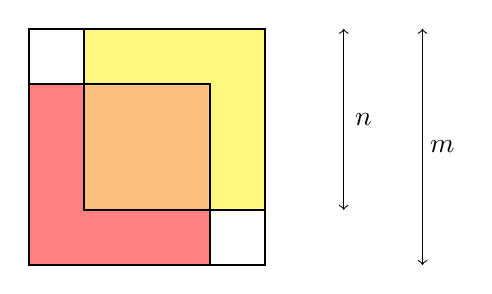
\begin{tikzpicture}
		\draw[thick] (0,0) rectangle (3,3);
		\draw[thick, fill=red!50] (0,0) rectangle (2.3,2.3);
		\draw[thick, fill=yellow!50] (0.7,0.7) rectangle (3, 3);
		\draw[thick, fill=orange!50] (0.7,0.7) rectangle (2.3, 2.3);
		\draw[<->] (4, 0.7)--(4, 3);
		\node at (4.25, 1.85) (n) {$n$};
		\draw[<->] (5, 0)--(5, 3);
		\node at (5.25, 1.5) (m) {$m$};
	\end{tikzpicture}
\end{center}
Omdat $m^2 = 2n^2$, is het stuk waar de twee vierkanten met zijde $n$
over elkaar liggen even groot als het stuk dat door geen van beide
vierkanten wordt bedekt. De oppervlakte van het oranje vierkant is dus
even groot als die van de twee niet-ingekleurde vierkanten samen. Noem de zijde van
het oranje vierkant $p$ en de zijde van elk niet-ingekleurd vierkant
$q$. Dan is $p^2 = 2q^2$. Maar nu is $\sqrt{2} = \nicefrac{p}{q}$,
waarbij $p < m$, $q < n$ en $p, q \in \Nat$. Dat kan niet: we hadden
$m$ en $n$ juist zo klein mogelijk gekozen.
\emph{De tweede manier is formeel.} Uit $m^{2} = 2n^{2}$
volgt dat $m$ even is. (Als $x$ oneven is, kun je makkelijk laten zien
dat $x^2$ ook oneven is.) Dus $m = 2r$ voor een bepaalde $r \in \Nat$. Als we dit
omwerken, krijgen we $2r^2 = n^2$,
		%				\begin{align*}
		%					(2q)^{2} &= 2n^{2}\\
		%					4q^{2} &= 2n^{2}\\
		%					2q^{2} &= n^{2}
		%				\end{align*}
dus ook $n$ is even. Zowel $m$ als $n$ is dus even. De breuk
$\nicefrac{m}{n}$ \emph{kan} daarom toch verder worden vereenvoudigd.
Dat is de tegenspraak.
\end{proof}
Dit bewijs met een plaatje brengt ons trouwens terug bij
\olref[his][set][mythology]{sec}. Tennenbaum (1927--2006) was beslist
een moderne wiskundige. Toch is het bewijs onmiskenbaar mooi en
helemaal waterdicht, en sluit het aan bij ons meetkundige gevoel.
Hoe dan ook: de reële getallen zijn ``uitgebreider'' dan de rationale
getallen. Je kunt zeggen dat de rationale getallen ``gaten'' hebben en
dat de reële getallen die opvullen. Weierstrass zag dat één eigenschap
precies dit verschil beschrijft. Die heet de volledigheidseigenschap:
\emph{Elke niet-lege verzameling reële getallen die een bovengrens
heeft, heeft ook een kleinste bovengrens.}
Je ziet makkelijk dat de rationale getallen deze
volledigheidseigenschap niet hebben. Neem bijvoorbeeld alle rationale
getallen kleiner dan $\sqrt{2}$:
\[
	\Setabs{p \in \Rat}{p^2 < 2 \text{ of }p < 0}
\]
Deze verzameling heeft binnen de rationale getallen een bovengrens.
Alle !!{element}en zijn bijvoorbeeld kleiner dan $3$. Maar wat is de
kleinste bovengrens? We willen `$\sqrt{2}$' zeggen, maar we hebben net
gezien dat $\sqrt{2}$ \emph{niet} rationaal is. Er is ook geen
\emph{kleinste} rationaal getal dat groter is dan $\sqrt{2}$. De
verzameling heeft dus wel een bovengrens, maar geen kleinste
bovengrens. Daarom hebben de rationale getallen de
volledigheidseigenschap niet.
Bij een ononderbroken getallenlijn, het continuüm, verwachten we juist
de volledigheidseigenschap. We willen niet alleen dat $\sqrt{2}$ een
reëel getal is. We willen alle ``gaten'' in de rationale getallenlijn
opvullen, zodat het continuüm zelf geen ``gaten'' meer heeft. Dat is
precies wat volledigheid ons zal geven.
\end{document}